% Generated by scripts/supp_tex.py from scripts/supp/h_limits.py.
% Do not edit: edit the module, which also builds the PDF version.

\section{Failure cases, limitations and open problems}
\label{supp:h_limits}

The method removes decoder compute by letting easy tiles leave the trunk early, and there are frames where no tile is easy, frames with too few tiles to allocate over, and content where the quality a budget buys is spent in a place a viewer would look. This section measures those cases rather than describing them, then lists the mechanisms that were built for this work and dropped, each with the measurement that ended it, and closes on the problems that are open at submission. Section D names five failure cases read off the operating-point files and is not repeated; what follows is the content axis, the abandoned work, and the state of the checkpoints every table in this document rests on.

\subsection{The frames it does worst on}

A frame is cut into tiles of 256 px, so the number of decisions the allocation has to make is fixed by the resolution. At 1920$\times$1080 a padded frame carries 40 tiles and at 416$\times$240 it carries two. Table 1 takes one frame from each of the five test classes at the same rate and the same budget and prints what the allocation did with it. Reading down the tile column, the exit map goes from a mixture over three exits to a constant, and the saving falls with it.

\begin{table}[t]
\centering
\resizebox{\columnwidth}{!}{%
\begin{tabular}{lrrrrr}
\toprule
frame & tiles & exits taken & saved \% & delivered dB & worst tile dB \\
\midrule
Bosphorus, 1920$\times$1080 & 40 & e2:29 e3:8 e4:3 & 34.2 & 0.099 & 0.374 \\
BasketballDrive, 1920$\times$1080 & 40 & e2:22 e3:9 e4:9 & 29.9 & 0.099 & 0.178 \\
FourPeople, 1280$\times$720 & 15 & e2:6 e3:1 e4:3 e5:5 & 19.6 & 0.100 & 0.271 \\
PartyScene, 832$\times$480 & 8 & e3:4 e4:3 e5:1 & 16.9 & 0.097 & 0.162 \\
RaceHorses, 416$\times$240 & 2 & e3:1 e4:1 & 18.6 & 0.095 & 0.134 \\
\bottomrule
\end{tabular}}
\caption{\textbf{One frame from each class at q32 and a 0.1 dB budget.} The exits taken column is the histogram over the ladder, so \emph{e4:2} is two tiles at exit 4. Take from it that the allocation stops being an allocation at the bottom of the table: at 416$\times$240 both tiles take the same exit, and the frame receives whatever that one rung happens to cost. The worst tile column is the largest per-tile loss in the frame and is between two and three times the frame's own delivered decibel on the three largest frames, which is the tail section D measures over the whole set.}
\end{table}

{\small The five results/supp\_exitmap\_*\_q32\_b01.json files, all on runs/RECIPE512/ckpt\_PAPER.pth.tar, one frame each. These probes carry the modelled saving and no hook count, so each is optimistic by up to 0.8 points, the constant recorded in results/ceiling\_measured.json; they are printed for the allocation and the per-tile loss rather than for the headline, which section D reports hook-counted over the whole set.}

\begin{figure}[t]
\centering

\includegraphics[width=\columnwidth]{figures/exitmap_PAPER_racehorses_416x240_q32_b01.png}
\caption{\textbf{The smallest frame in the test set, and the whole of its allocation.} \textbf{a}, the decoded frame with the single tile boundary drawn, tinted by the exit each tile took. \textbf{b}, the exit map, two cells. \textbf{c}, the loss each tile pays. Both tiles take exit 4 and the map has nothing to trade; the legend gives what each rung would have saved had a tile taken it.}
\end{figure}

{\small paper/figures/exitmap\_PAPER\_racehorses\_416x240\_q32\_b01.png, drawn from results/supp\_exitmap\_racehorses\_416x240\_q32\_b01.json on runs/RECIPE512/ckpt\_PAPER.pth.tar. RaceHorses at 416$\times$240, q32, 0.1 dB.}

The two frames at either end of that table are the same decoder at the same budget. Bosphorus at 1080p spreads 40 tiles over exits 2, 3, 4 and saves 34.2\% of the modelled decode; RaceHorses at 416$\times$240 puts both of its tiles on exit 4 and saves 18.6\%. Nothing about the content separates them. What separates them is that a two-cell map has three admissible states above the split depth and a 40-cell map has more states than the sweep could enumerate, so the Lagrangian has somewhere to put the budget in one case and not in the other.

\begin{table}[t]
\centering
\resizebox{\columnwidth}{!}{%
\begin{tabular}{lrrrrrr}
\toprule
sequence & q & tiles & PSNR lost dB & MS-SSIM lost dB & saved \% & its rank \\
\midrule
videoSRC26 & q0 & 40 & 0.137 & 0.118 & 39.1 & 49th \\
KristenAndSara & q0 & 15 & 0.162 & 0.111 & 37.1 & 26th \\
videoSRC03 & q0 & 40 & 0.147 & 0.107 & 37.4 & 28th \\
\bottomrule
\end{tabular}}
\caption{\textbf{The three sequences that lose most on the perceptual metric.} All three are 1080p frames at the lowest rate and carry the full 40 tiles. The MS-SSIM column is $-$10 log10(1 $-$ MS-SSIM), the unit section D puts the two metrics in, and on these sequences it is two to three times the set mean of 0.050 dB at this rate. The PSNR column is the same file's own difference in PSNR and runs from 0.137 to 0.162 dB, over the nominal budget on all three, which is the per-sequence overshoot the next subsection measures. The last column is where each sits in the set by compute saved, from the 26th percentile to the 49th: these are not the sequences that save least.}
\end{table}

{\small The worst\_sequences\_by\_ms\_ssim block of results/supp\_opquality\_PAPER.json, on runs/RECIPE512/ckpt\_PAPER.pth.tar, \NumSeq sequences at one frame each, at the 0.1 dB operating point of results/supp\_paper\_curve\_PAPER.json. That block is the file's own shortlist of the fifteen largest MS-SSIM losses over the whole sweep, reordered here by the decibel rather than by the raw difference. The saving column is the same file's per-sequence saving against our own deepest exit and the rank is its percentile among the \NumSeq sequences of results/supp\_per\_sequence\_PAPER\_b010.json at the same rate.}

The ordering there is the one to take away. A budget in PSNR does not price the second metric evenly across content, and the sequences where the two disagree most are ordinary 1080p clips from the middle and upper part of the set by saving rather than the hard cases further down this section. On a clip with 40 tiles the multiplier can move a third of the frame two rungs down the ladder and stay inside 0.1 dB of PSNR, and the tiles it moves are the flat, low-texture ones a structural metric weighs differently from a mean squared error. The remedy is a budget written in the metric a deployment cares about, and no allocation in this work was bisected on anything but PSNR.

\subsection{What a set-level budget hides}

\begin{table}[t]
\centering
\resizebox{\columnwidth}{!}{%
\begin{tabular}{lrrrrr}
\toprule
q & over budget & worst dB & on & least saved \% & on \\
\midrule
q0 & 32 of 53 & 0.248 & Jockey & 24.2 & BQSquare \\
q16 & 33 of 53 & 0.243 & videoSRC02 & -1.0 & BQSquare \\
q32 & 31 of 53 & 0.258 & videoSRC02 & -1.0 & BQSquare \\
q48 & 31 of 53 & 0.253 & videoSRC02 & -1.0 & BlowingBubbles \\
q63 & 31 of 53 & 0.215 & videoSRC02 & -1.0 & BQSquare \\
\bottomrule
\end{tabular}}
\caption{\textbf{The 0.1 dB budget, sequence by sequence.} The multiplier is bisected once for the whole set, so the budget binds on the set mean and on nothing else. Rather more than half the sequences receive a decode worse than the budget they were nominally given, and the worst of them receives between two and three and a half times it. Section D.4 gives the spread on the compute axis; this is the same allocation seen on the quality axis.}
\end{table}

{\small results/supp\_per\_sequence\_PAPER\_b010.json, the rows block for the delivered decibel and rows\_vs\_release arithmetic for the saving, on runs/RECIPE512/ckpt\_PAPER.pth.tar. Decibels are pooled, the convention results/supp\_paper\_curve\_PAPER.json bisects in.}

\textbf{The budget is spent unevenly across the colour components.} Every quality number in this work is DCVC-UF's own 6:1:1 weighted YUV420 PSNR, in which chroma carries an eighth of the weight, and the budget is set on it. Split into its parts at the 0.1 dB budget, luma falls by 0.066 dB and the two chroma planes by 0.205 and 0.223 -- chroma loses 3.3 times what luma loses. The weighted mean lands on the budget exactly as it is supposed to, and says nothing about the split underneath it.

\begin{table}[t]
\centering
\resizebox{\columnwidth}{!}{%
\begin{tabular}{lrrrr}
\toprule
budget & PSNR-Y & PSNR-U & PSNR-V & 6:1:1 \\
\midrule
0.1 dB & -0.066 & -0.205 & -0.223 & -0.103 \\
0.2 dB & -0.108 & -0.399 & -0.439 & -0.186 \\
0.3 dB & -0.126 & -0.468 & -0.525 & -0.218 \\
0.5 dB & -0.126 & -0.468 & -0.525 & -0.218 \\
\bottomrule
\end{tabular}}
\caption{\textbf{Quality given up per colour component}, dB below the released decoder, averaged over the five rates on the \NumSeq test frames. The last column is the metric the budget is set on; the first three are what it is made of.}
\end{table}

{\small results/rd\_yuv\_PAPER.json. The operating points are not re-derived: each row of the signalled sweep records the multiplier its bisection settled on, and the exit map is a deterministic argmin given that multiplier, so the decode measured here is the decode the sweep priced. The split is checked against the weighted figure on every frame.}

The mechanism is the objective, not the ladder. The allocation minimises absolute error, and chroma starts with far less of it -- at the lowest rate the released decoder reaches 38.9 dB on U against 30.2 on Y, so chroma's mean squared error is about seven times smaller. The same absolute increase is therefore a much larger number of decibels on chroma, and an allocator that does not know the difference spends it there first. A budget set on the weighted metric cannot see this; one set per component could, and that is the change we would make.

\begin{figure}[t]
\centering
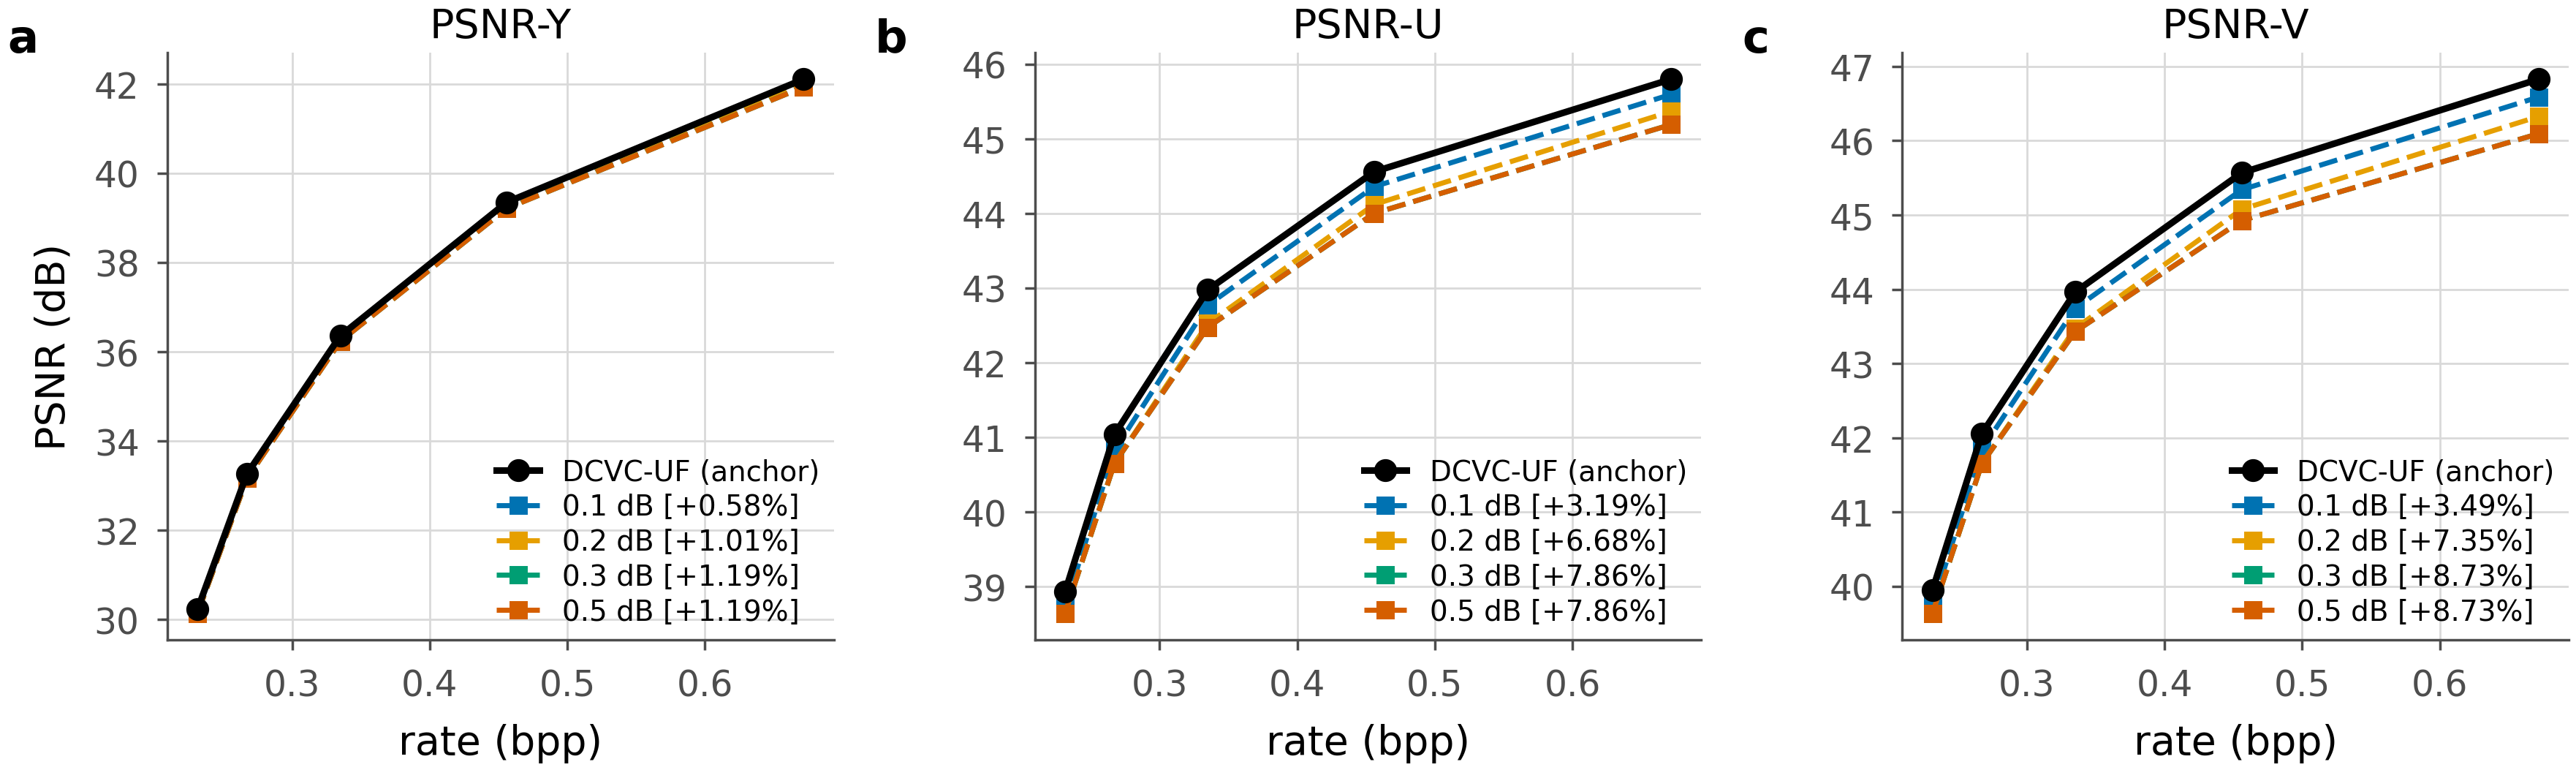
\includegraphics[width=\columnwidth]{figures/rd_yuv.png}
\caption{\textbf{Rate-distortion per colour component}, ours against the released decoder, one panel per component, with each budget's BD-rate against the anchor in brackets. The anchor is the released decoder on the same bitstream, so a bracket is the price of decoding one file with fewer operations rather than one codec against another.}
\end{figure}

The other thing a set mean hides is how much of the budget is gone before any tile exits early. With every tile at full depth the decode already differs from the released decoder by 0.022 dB at q0 and 0.048 dB at q63, which is two thirds of the headline budget at the high rate. Two things make it up, and they are measured separately rather than subtracted from one another: the deepest exit's own departure from the released decoder, 0.028 dB at q63 on the same checkpoint, and the seam left by cutting the frame into tiles. Both are charged to the method, because the saving is measured against the released decoder rather than against our own full-depth decode, and both grow with rate while the budget does not.

{\small Floors from results/signalled\_RECIPE512\_ctc53.json and drift from results/supp\_anchor\_PAPER.json, both on runs/RECIPE512/ckpt\_PAPER.pth.tar over \NumSeq sequences. The two files do not pool their decibels alike, which is why the seam is described rather than given as the difference. Section C derives why a floor above the budget makes the feasible set empty and section E tabulates the three ways the floor itself can be measured.}

\begin{figure}[t]
\centering

\includegraphics[width=\columnwidth]{figures/seam_PAPER_bosphorus_q63.png}
\caption{\textbf{The seam, at frame scale.} \textbf{a}, the decoded frame. \textbf{b}, the absolute error against a full-frame decode of the same latent, amplified 30$\times$, with every tile at the deepest exit so that nothing here is early exiting. \textbf{c}, a zoom on one junction. The tile grid is the error: 0.136 dB at q63, paid before the allocation begins.}
\end{figure}

{\small paper/figures/seam\_PAPER\_bosphorus\_q63.png, drawn from results/supp\_seam\_problem\_bosphorus\_q63.json on runs/RECIPE512/ckpt\_PAPER.pth.tar. The panel is the worst case rather than the shipped one: the file records tile\_pad\_mode zeros with the deblocking filter removed, which is how the artefact is made visible. The floors quoted above are the shipped configuration, replicate padding with the filter on.}

\subsection{Built, measured and abandoned}

Seven mechanisms were built, measured and then left out of the reported system. Two of them replace the border a tile is convolved against, one repairs the seam afterwards, one removes the seam by letting neighbouring tiles exchange features, one freezes the trunk so that the deepest exit cannot move, one gives the small resolutions a smaller tile, and the last is an explanation of the tiling penalty rather than a mechanism. Table 5 gives what settled each, and the file it was settled in. The cost of building them is not otherwise recoverable from the paper, and two of them are the first thing a reader would propose.

\begin{table}[t]
\centering
\resizebox{\columnwidth}{!}{%
\begin{tabular}{lr}
\toprule
what was built & the measurement that ended it \\
\midrule
First-order border extrapolation & worse than replication at all three rates: 0.198, 0.286 and 0.384 dB against 0.071, 0.123 and 0.218 \\
Fitted AR(1) border padding & ahead of replication by 0.021 dB at q63, and bought with wall clock that no file in results/ records \\
A learned deblocking filter & 0.0008 dB even with a perfect gate, against 1.09\% of a decode \\
Halo exchange between tiles & exact at uniform depth, and the saving falls from 31.2\% to 5.5\% at q32 and from 28.0\% to 1.0\% at q63 \\
Freezing the trunk & drift exactly 0.000 dB, and the oracle ceiling collapses with it to 11.5\% at q0, 0.4\% at q32 and -1.0\% at q63 \\
A tile size chosen per resolution & worth -0.06 points on the set mean over three rates, with the training confound running in its favour \\
The affected-area fraction & wrong by 160 to 264\%, against 12 to 22\% for a power law in the per-tile block count \\
\bottomrule
\end{tabular}}
\caption{\textbf{Seven mechanisms and what settled each.} Five were built and dropped, one is a proposed extension measurement did not support, and the last is an explanation of the tiling penalty that the measurement does not carry. None of the seven is in the reported system, whose configuration is replicate padding at 256 px with the deblocking filter left on, as the ablation table of section A records.}
\end{table}

{\small Rows in order: results/ctc\_seam\_p256.json (40 sequences, three rates); the same file with results/shrink\_ablation.log; results/seam\_spatial\_published.json with the module's share of a decode from results/supp\_module\_shapes.json; results/coupling\_ablation.json; results/first\_ckpt\_headsonly.log; results/tilesize\_adaptive.json; results/supp\_seam\_vs\_split.json, refitted in the build. The coupling and heads-only files are on runs/RECIPE512/ckpt\_eval.pth.tar and runs/heads\_only\_j2\_p256/ckpt\_epo0.pth.tar; the seam-repair spatial file is on a runs/BEST checkpoint whose epoch it does not record. The rest are on runs/RECIPE512/ckpt\_PAPER.pth.tar.}

Three of those rows need more than a line. The halo exchange does two of the three things asked of it: it is exact at uniform depth, and it removes 100\% of the floor at q0 and 43\% at q63. The third, that closing the floor is worth several points of saving, has the wrong sign at every rate above the lowest. A tile whose neighbour ran six more blocks is reading an activation the trained weights have never seen, and the error that introduces is far larger than the seam it removed. Exactness holds when every tile is at the same depth, and routing is the deliberate violation of that condition, so the two are in tension by construction. The one caveat that keeps this from being final is that the model was trained with replicate padding, so switching the exchange on at inference is a distribution shift; a run trained with it could reverse the sign, and no such run exists.

The deblocking filter is the reverse case, where the mechanism does what it was built to do and the amount is too small to pay for. Error falls monotonically with distance from the nearest tile boundary, 4.7e-05 in the innermost 4 px against 4.1e-05 more than 64 px away, so the seam is real and it is local. The filter's gate leaks: it gains in the boundary band and loses slightly everywhere else. Giving it a perfect gate, with its boundary gain kept and its interior loss set to zero, bounds it at 0.0008 dB for 1.09\% of a decode. Tightening the gate cannot rescue the module because there is not enough in the band for it to win. It is still switched on in the reported system, because it was trained jointly with the decoder and switching it off at inference is not the same experiment as training without it, and no run has been trained without it at 256 px.

The affected-area fraction is an explanation rather than a mechanism, and it is the weaker of the two available. It is a correct statement about which pixels a tile border can reach and a poor predictor of what the border costs, because it saturates: at 12 blocks per tile it is already 0.94 and cannot rise further, while the penalty still climbs by a factor of 3.1 from 8 blocks to 12. Fitted with one free scale it is wrong by 160 to 264\% on average. A power law in the block count is wrong by 12 to 22\%, with exponents 2.38, 2.22 and 1.93 at q0, q32 and q63 and log-log correlations from 0.979 to 0.995. An exponent near two has a reading: the number of affected pixels grows with the border's reach and the damage in each grows with how many convolutions reached it, and the two are the same quantity. The drift from 2.38 to 1.93 with rate is not explained here. The control is the row that licenses reading any of it as seam: at zero blocks per tile the penalty is 0.0000 dB at every rate.

The tile-size row is the one a reader is most likely to propose, since the exit maps of Table 1 say the method is governed by tile count. Splicing 128 px tiles into the two smallest classes and leaving 256 px elsewhere is worth -0.06 points on the set mean, averaged over three rates. The direction differs by rate rather than being uniformly flat: at q0 the smaller tile is ahead in five of six classes and the splice gains +0.33 points, while at q63 the smaller tile is behind on every class and the splice loses -0.33. Halving the tile side doubles the seam at fixed depth, and above the lowest rate the extra seam costs more than the extra granularity returns. The comparison is not matched for training time: the 128 px column carries 24,000 more steps than the pinned checkpoint, an advantage that runs in the smaller tile's favour, which is why the conclusion is that the extension is not supported rather than that it is harmful.

{\small results/tilesize\_adaptive.json, which splices results/per\_class\_RECIPE512.json on runs/RECIPE512/ckpt\_PAPER.pth.tar against results/per\_class\_BEST128.json on runs/BEST128/ckpt\_step.pth.tar. The file brackets the training confound with a third measurement on runs/RECIPE512/ckpt\_PIN\_e1.pth.tar and records the verdict per class and per rate.}

The AR(1) padding row is the one this section cannot close from results/. It is the best border estimator measured, 0.197 dB at q63 against 0.218 for replication, and it was rejected on wall clock, which no file in results/ holds. What results/ does hold is why nothing cheaper works. Its coefficient is fitted per channel and per tile, and replacing the fit with a fixed shrinkage recovers none of the gain: at a coefficient of 0.95 the seam is 0.2138 dB against replication's 0.2160 and the fit's 0.1797, and every coefficient below that is worse than replication at every rate. The gain is in the adaptivity, and the adaptivity is what costs.

{\small results/shrink\_ablation.log, 10 CTC frames at j = 2 and 128 px, typed into this module because it is a log rather than JSON; the seam figures it is compared against are results/ctc\_seam\_p256.json, 40 sequences at 256 px, so the two sets of absolute values are not on one protocol and only the ordering within each is read. The wall-clock measurement that decided the estimator is recorded in the project's decision log and in no file in results/.}

\begin{figure}[t]
\centering

\includegraphics[width=\columnwidth]{figures/seam_module.png}
\caption{\textbf{The learned deblocking filter, and where it wins.} It is gated by position within a tile and applied once to the stitched frame, for 1.09\% of the decode. \textbf{a}, the trained gate against distance from the boundary, beside its initialisation. \textbf{b}, the change in error by that distance; bar width is the share of pixels, so bar area is the contribution to the frame. It wins on the pixels nearest a boundary and loses on the rest, which is why a perfect gate still cannot pay for it.}
\end{figure}

The exactness claim for the halo exchange is worth writing out, because it is the condition and not the number that carries the argument. At uniform depth the largest absolute difference between a tiled decode with the exchange and a full-frame decode of the same latent is exactly zero once the deblocking pass is switched off; with the pass on it is 4.27e-02, because that pass runs on the stitched frame and has no full-frame counterpart, and with replicate padding instead of the exchange it is larger again. The condition in that sentence is \emph{uniform depth}, and routing is the deliberate violation of it, which is the whole of the tension.

\begin{figure}[t]
\centering
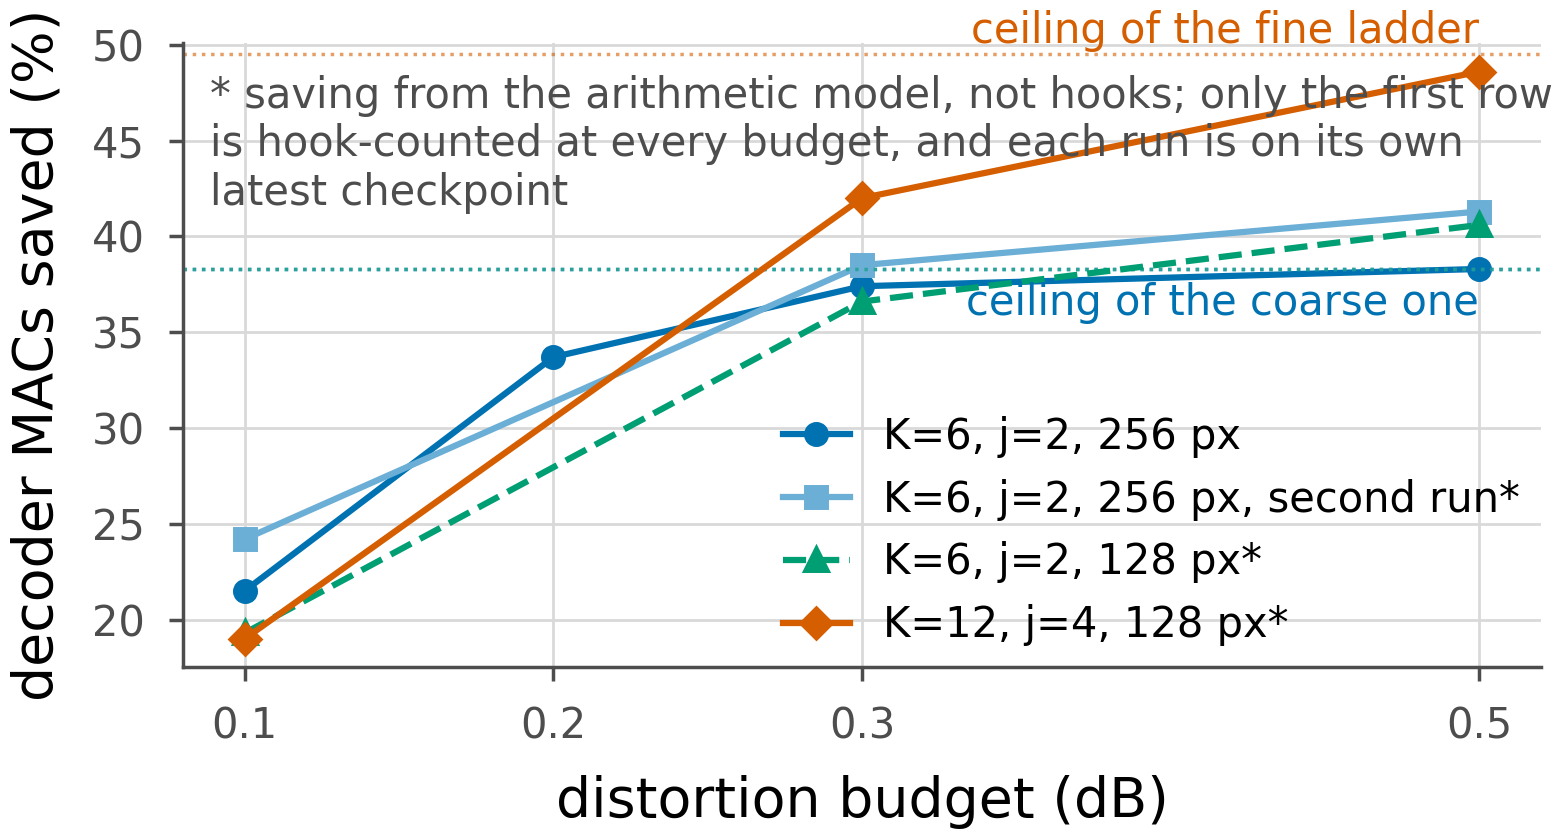
\includegraphics[width=\columnwidth]{figures/ladder_crossover.png}
\caption{\textbf{The right ladder depends on the budget.} Saving against budget for four ladders, with each one's architectural ceiling as a dotted line. A finer ladder has a higher ceiling and a higher floor, so the curves cross: the coarse ladder wins where the budget is tight and cannot be spent, and the fine one wins where it is loose enough to reach exits the coarse ladder does not have. The crossing is the design choice this section is about. }
\end{figure}

\begin{figure}[t]
\centering
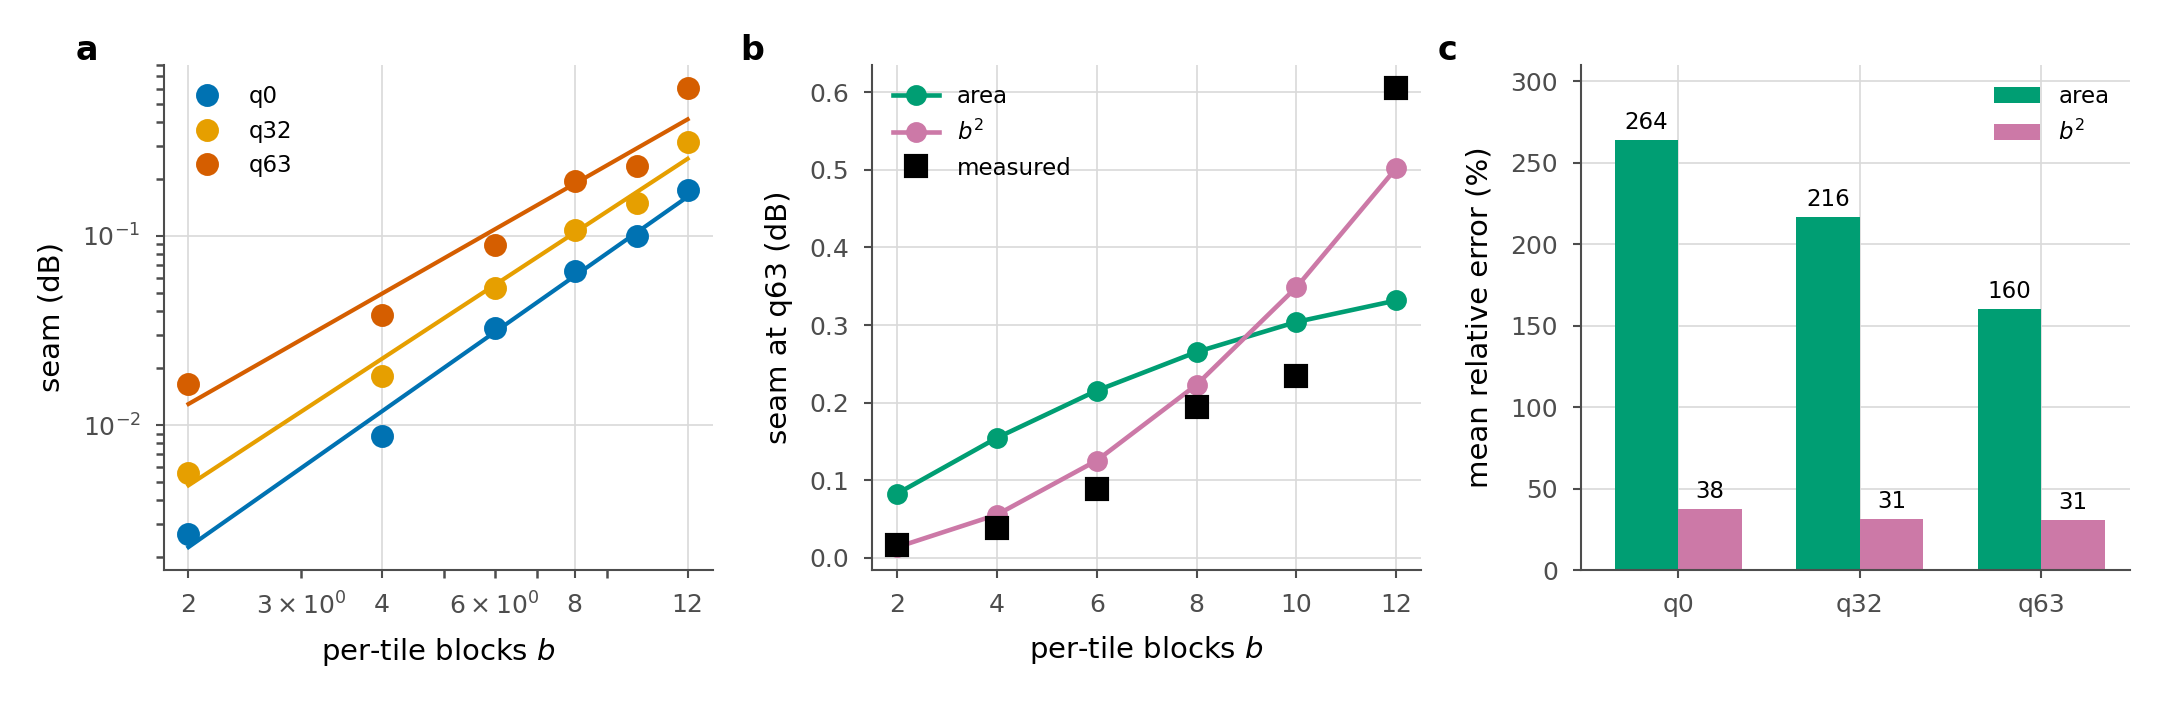
\includegraphics[width=\columnwidth]{figures/contamination.png}
\caption{\textbf{The seam against per-tile depth.} \textbf{a}, the measurement with the fitted power law. \textbf{b}, both models against q63, one free scale each. \textbf{c}, mean relative error. The area fraction saturates once the border reaches every pixel and the penalty does not, which is where the area law fails as a predictor.}
\end{figure}

\subsection{The checkpoints, and what a later one measures}

Every table in this supplement is measured on runs/RECIPE512/ckpt\_PAPER.pth.tar, taken at the end of epoch 4. The per-checkpoint watcher measured the earlier epochs of the same run on the same \NumSeq sequences at the same budget through the same code path, and Table 6 is what they say.

\begin{table}[t]
\centering
\resizebox{\columnwidth}{!}{%
\begin{tabular}{lrrrrrr}
\toprule
checkpoint & q0 & q16 & q32 & q48 & q63 & mean \\
\midrule
RECIPE512, epoch 0 & 29.2 & 25.0 & 20.3 & 17.8 & 15.2 & 21.5 \\
RECIPE512, epoch 1 & 30.1 & 26.4 & 21.4 & 19.4 & 16.8 & 22.8 \\
RECIPE512, epoch 2 & 32.8 & 28.1 & 22.5 & 19.9 & 16.9 & 24.0 \\
RECIPE512, epoch 3 & 33.2 & 29.5 & 24.2 & 22.4 & 19.9 & 25.8 \\
RECIPE512, epoch 4, pinned & 33.7 & 30.1 & 26.1 & 24.8 & 23.5 & 27.6 \\
RECIPE512, epoch 5 & 34.3 & 30.8 & 26.1 & 24.8 & 23.4 & 27.9 \\
BEST, epoch 1 & 34.0 & 27.7 & 22.3 & 19.8 & 17.2 & 24.2 \\
BEST, epoch 2 & 29.4 & 23.2 & 18.0 & 14.5 & 11.5 & 19.3 \\
BEST, epoch 3 & 30.8 & 24.7 & 19.2 & 15.6 & 12.2 & 20.5 \\
\bottomrule
\end{tabular}}
\caption{\textbf{Compute saved at the 0.1 dB budget as training continues.} RECIPE512 and BEST are two runs of one configuration, same architecture and same recipe, differing only in the draw. The pinned row is what the paper reports, and it is the last epoch the run had completed when we stopped. Every RECIPE512 row is hook-counted on the same \NumSeq sequences, so the differences between them carry no convention offset. The series rises at every rate and at every step -- 21.5\% to 27.9\% on the set mean -- and the gain is larger at the high rates than the low ones, which is where the method had the least to give: q63 moves by 8.3 points against 5.2 at q0. Nothing here has flattened.}
\end{table}

{\small The RECIPE512 rows are every results/signalled\_RECIPE512\_*.json over the full \NumSeq set that carries a hook count, one row per epoch, selected by savings.epoch\_series -- the same rule the main paper's macros and the plateau figure use. The BEST rows are results/signalled\_BEST\_ctc53.json, results/signalled\_BEST\_0819\_1050.json and results/signalled\_BEST\_0820\_0841.json on the ckpt\_eval and ckpt\_step files of that run, which the watchers overwrite; each records its own epoch. None of the three carries a hook count, so they are on one basis with each other and about 0.8 points optimistic against every RECIPE512 row. Comparisons within either block carry none of that offset; comparisons across the two do.}

One condition governs any comparison between measurements made at different times. The test set grew from 40 sequences to 53 when MCL-JCV and the two smallest HEVC classes were added, and eight tiles at 832$\times$480 or two at 416$\times$240 save nothing like a 1080p frame does, so a saving measured on the smaller set is several points above one measured on the larger at the same checkpoint. Every row of this section is on \NumSeq sequences.

\subsection{How far two runs of one recipe are apart}

RECIPE512 and BEST are the same K, the same split depth, the same tile size, the same adapters and the same 45,445,398 parameters. At epoch 2 they are 4.7 points apart on the set mean. The ladder table of the main paper reports a 256 px run at 24.2 against a 128 px run at 19.3 and a twelve-exit run at 19.0, the last over the four rates it reaches rather than five, which are differences of about five points. The gap between two runs of one configuration is the same size as the architectural differences the table is ranking.

{\small results/signalled\_BEST\_ctc53.json, results/signalled\_BEST128\_ctc53.json and results/signalled\_FINE12\_ctc53.json, the three files behind the main paper's ladder table, each on the ckpt\_eval or ckpt\_step file of its own run; none of the three carries a hook count, so the three are on one basis with each other and about 0.8 points optimistic against the pinned row of Table 6. The epoch-2 comparison above is between two files that both carry one.}

The spread is not only between runs. The watcher writes a measurement every time it finds a new checkpoint, so one epoch of one run yields several, and Table 7 prints six of them from a single epoch. They span 1.8 points on the four-rate mean and up to 3.0 at a single rate, on one test set, one budget and one code path, with every row hook-counted.

\begin{table}[t]
\centering
\resizebox{\columnwidth}{!}{%
\begin{tabular}{lrrrrr}
\toprule
checkpoint, in order & q0 & q16 & q32 & q48 & mean \\
\midrule
0819\_0923 & 30.3 & 24.8 & 16.9 & 10.8 & 20.70 \\
0819\_1239 & 28.9 & 22.9 & 18.2 & 12.4 & 20.60 \\
0819\_1555 & 30.8 & 25.3 & 18.3 & 12.6 & 21.74 \\
0819\_1911 & 30.1 & 23.5 & 18.0 & 12.2 & 20.94 \\
0819\_2157 & 31.5 & 25.6 & 18.8 & 13.7 & 22.38 \\
0819\_2227 & 31.0 & 25.9 & 18.4 & 12.4 & 21.94 \\
\bottomrule
\end{tabular}}
\caption{\textbf{Six checkpoints from one epoch of one run.} FINE12 is the twelve-exit ladder, whose highest rate has no admissible allocation at this budget, so the mean is over the four rates that do. Take from it that a comparison at a matched epoch is not a comparison at a matched checkpoint, and that the difference between two rows here is as large as several of the differences this work reads as results.}
\end{table}

{\small The six results/signalled\_FINE12\_0819\_*.json files listed in this module, all at epoch 2 of runs/FINE12 on \NumSeq sequences at a 0.1 dB budget, all carrying a hook count. The checkpoints themselves are the run's own per-epoch files, which it rewrites, so these measurements are what preserve them. A seventh epoch-2 measurement is excluded because it carries no hook count.}

What follows from the two tables is a constraint on how this work may be read. No configuration was trained twice at two seeds, and no seed is set in the decoder's trainer, so there is no interval on any architectural comparison in this document. Section A says so and gives the sources of variation; what these files add is a magnitude. Until a configuration is trained twice, a difference of a few points between two rows of the ladder table is not separable from the difference between two runs of either of them.

\subsection{Anchor drift}

\begin{table}[t]
\centering
\resizebox{\columnwidth}{!}{%
\begin{tabular}{lrrrr}
\toprule
run & q0 & q32 & q63 & frames \\
\midrule
RECIPE512, pinned & 0.0004 & 0.0114 & 0.0283 & 53 \\
RECIPE512, epoch 0 & 0.0051 & 0.0145 & 0.0362 & 53 \\
BEST & 0.0015 & 0.0088 & 0.0154 & 53 \\
BEST128 & 0.0036 & 0.0104 & 0.0216 & 53 \\
FINE12 & 0.0075 & 0.0245 & 0.0602 & 53 \\
VERBATIM, no anchor term & 0.1101 & 0.1241 & 0.1594 & 40 \\
\bottomrule
\end{tabular}}
\caption{\textbf{How far the deepest exit has moved from the released decoder}, in decibels, one checkpoint per run. The deepest exit is supposed to be the released decoder and the training objective carries a term that holds it there. The term does real work: the run trained without it sits 0.110 to 0.159 dB away, more than the whole headline budget at every rate before a single tile has exited early. The term does not hold it exactly, and what it leaves behind grows with rate: 28\% of a 0.1 dB budget at q63 on the pinned checkpoint and 60\% on the twelve-exit run, whose floor exceeds that budget outright at the highest rate.}
\end{table}

{\small results/supp\_anchor\_PAPER.json on runs/RECIPE512/ckpt\_PAPER.pth.tar; results/anchor\_RECIPE512\_e0.json is the same measurement on the same frames and rates when the pin held epoch 0 of that run; results/anchor\_BEST.json, results/anchor\_BEST128.json, results/anchor\_FINE12.json and results/anchor\_VERBATIM.json on the ckpt\_eval or ckpt\_step file of their runs, at the epoch each happened to be at, which none of them records. Frame counts differ by file and are printed, because two of these are 40 frames and are not comparable with the \NumSeq-frame rows at the fourth decimal.}

Whether it grows with training is now settled, on this run at least. The two RECIPE512 rows are four epochs apart on the same \NumSeq frames and the same rates, and the drift falls at 5 of the 5: 0.0051 to 0.0004 dB at q0 and 0.0362 to 0.0283 at q63. The anchor term tightens its hold as the run goes on rather than losing it, which is the direction the term is there to produce and not one we had evidence for before. It does not fall evenly. At q0 the drift is down to 0.0004 dB, which is where this measurement stops resolving it; at q63 it fell by 22\% and is still 0.0283. The ratio between the two ends is therefore not worth quoting, and the direction with rate is what survives the move. The open problem is the size at the top of the ladder, not the trend: at q63 28\% of a 0.1 dB budget is spent before the allocation begins, and a move to any later checkpoint has to remeasure this and report it as its own row rather than assume it carries over.

There is a structural fix and it was measured and rejected, which is row five of Table 5. Freezing the trunk makes the deepest exit the released decoder by construction, with no weight left that could move, and the drift measures exactly zero. The shallow exits then cannot improve either, because the exit heads alone cannot recover what six skipped blocks contained, and the oracle ceiling collapses to nothing above the lowest rate. Training the trunk is what makes the ladder worth having, and the drift is what training the trunk costs.

\subsection{How much of this can be repeated exactly}

Every measurement file records the checkpoint it was taken on, and there are three kinds of answer. 71 of the files these two documents read name a checkpoint that does not move -- a pin or a warm start -- so the measurement can be repeated exactly. Another 17 name one the watcher overwrites but record the epoch or step it was at, so the weights are identified even though the path is not. The remaining 10 record neither, and their paths now point at whatever those runs have trained to since.

That last group is not hidden -- several of the files in it are named as such where they are used, and the epoch tables of this section exist because of it -- but it is worth stating once as a number rather than as remarks. Nothing in the main paper's headline is in it: the pinned checkpoint carries every table the paper reports. What is in it is the adapter and coupling ablations, the hybrid sweeps of configuration C, the wall-clock files and the anchor drift of the runs other than the pinned one. Repeating those exactly would need the checkpoints back, which is why scripts/check\_provenance.py refuses to let the count grow.

{\small Counted in the build over results/*.json against the file names scripts/build\_pdf.py, scripts/make\_paper\_tables.py and scripts/supp/*.py mention. The same count is a check, with the present figure of 10 as its baseline.}

\subsection{What is open}

Every open problem in this supplement is listed here, so that a reader meets each of them once. Section A gives the provenance of each table and section D the spread behind each mean; what follows is what those two cannot close.

\begin{itemize}\itemsep1pt
\item \textbf{The reported checkpoint is early.} Table 6 says a later checkpoint of the same run saves more at every rate. Nothing in this document is measured on one, because \NumClaims checked claims, every table and every figure rest on the pinned checkpoint, and moving it means remeasuring all of them. What a later checkpoint would change is the size of the headline and the anchor drift beneath it, in opposite directions.
\item \textbf{No interval exists on any architectural comparison.} Two runs of one configuration are 4.7 points apart at a matched epoch, and six checkpoints inside one epoch of one run span 1.8. Both are the size of the differences the ladder table ranks. The remedy is repeated runs, which is a training cost this work has not spent.
\item \textbf{The anchor is held by a loss term and not by construction.} The deepest exit is 0.028 dB from the released decoder at q63 on the pinned checkpoint, about a third of the headline budget, and the one construction that removes the drift removes the ladder's value with it.
\item \textbf{Everything here is one decoder's intra path.} The ladder is built inside the intra decoder of one released codec and measured on intra frames of video sequences at 1080p and below. No inter frame, no second codec rearranged into a ladder, and no resolution above 1080p, the last because the evaluation card has about 5 GB free and a 4K decode does not fit. The construction needs a residual trunk with a shared head and nothing else, which is an argument rather than a measurement.
\item \textbf{The window is measured with the losses known.} The allocations in this section are the exact per-tile search, which bounds any decoder-side predictor. Section F measures how much of it a trained head reaches and how much a rule with no learned parameters reaches, and neither closes the gap at high rate.
\item \textbf{Part of the recipe is pinned outside results/.} Nothing that writes to results/ runs inside the trainer, so the hyperparameter table of A.11, the dataset statistics of A.8 and the training wall clock are read from the launcher, the trainer and the run's own log rather than from a measurement file. The warm-start report on disk is the K = 12 rebuild rather than the K = 6 one the pinned run descends from; its two zero-difference controls are asserted at every build instead, so a failure would stop the run.
\item \textbf{One accelerator class.} Every millisecond and every joule in this work is an NVIDIA RTX A6000, all eight cards in this machine being that model, and the CPU rows of section B are the only second device class. Power comes from the driver counter, with no external meter to calibrate it against.
\end{itemize}

No internal check is outstanding. They all hold, including the one this list would otherwise have carried: the partially signalled configuration reduces to the fully signalled one to four decimals when every tile is overridden, with both sides read in the same saving convention, so the cost model's 0.8-point offset cannot present itself as a failure of the interpolation. As recorded in results/check\_paper.json, 88 of 88 checked claims pass.

